\documentclass{article}

\usepackage{graphicx} 
\usepackage{amsmath}
\usepackage{amssymb}
\usepackage{caption}
\usepackage{subcaption}
\usepackage{hyperref}
\usepackage{listings}
\usepackage{xcolor}
\usepackage{booktabs}

\definecolor{codegreen}{rgb}{0,0.6,0}
\definecolor{codegray}{rgb}{0.5,0.5,0.5}
\definecolor{codepurple}{rgb}{0.58,0,0.82}
\definecolor{backcolour}{rgb}{0.95,0.95,0.92}

\lstdefinestyle{mystyle}{
    backgroundcolor=\color{backcolour},   
    commentstyle=\color{codegreen},
    keywordstyle=\color{magenta},
    numberstyle=\tiny\color{codegray},
    stringstyle=\color{codepurple},
    basicstyle=\ttfamily\scriptsize,
    breakatwhitespace=false,         
    breaklines=true,                 
    captionpos=b,                    
    keepspaces=true,                 
    numbers=left,                    
    numbersep=5pt,                  
    showspaces=false,                
    showstringspaces=false,
    showtabs=false,                  
    tabsize=2
}

\lstset{style=mystyle}
\title{Transformer applied to Facial Landmark detection}

\author{Francesco Bertolotti}

\date{\today}

\begin{document}
\maketitle
\newpage
\section{Introduction}\label{sects:introduction}

One of the most popular deep learning (DL) architectures for natural language processing (NLP) is the Transformer architecture. The Transformer was popularized in the famous paper "Attention is all you need" \cite{Vaswani17}. From the original proposal, many architectural improvements have been proposed, e.g. \cite{Devlin18, Liu19, Yang19} and many others. Recently, the Transformer is being applied also to task for which wasn't originally designed. One notable example is image processing. In particular, \cite{Dosovitskiy20} adapt the Transformer architecture to process images. This represents one of the firsts instances of convolution-free architecture to achieve comparable results with the state-of-the-art (SOTA). The same idea is further explored in \cite{Wang21} using a pyramidal-like Transformer architecture. This architecture achieves further improvements surpassing results obtained by ResNets architectures \cite{He16}. While the Transformer architecture is gaining further traction in image processing tasks the potentialities remain mostly unexplored. With this project, we aim to apply and adapt the Transformer for the task of "Facial Landmark Detection". While most of the previous works aim to convolution-free architectures, we aim to combine the ResNets and the Transformers hoping to gain further improvements.


\section{Vision Transformer}\label{sects:Transformer}
In this sections, we are going to expose the inner workings of the Transformer architecture. Firstly, let us start by the input. The Transformer takes as input $n$ embeddings of size $d$. In our case, embeddings will be patches of an image, as shown by the Fig.~\ref{img:patches}. Let us call $X = [x_1, \dots, x_n] \in \mathbb{R}^{n\times d}$. Now that we have our patches, we can feed them to the first Transformer Encoder layer. Let us introduce three parameter matrices $W_Q, W_K, W_V \in \mathbb{R}^{n\times d}$. We proceed to compute the so called quries, keys and value vectors:
\[Q = X^T\cdot W_Q, K = X^T\cdot W_K, V = X^T\cdot W_V\]
Once we have computed these matrices representing three different linear transformation of the input, we proceed by applying the so called self-attention. But firstly, let us introduce the softmax non-linearity. The softmax function takes as input a vector $v \in \mathcal{R}^{1\times k}$ and outputs a vector $v' \in \mathcal{R}^{1\times k}$ such that $\sum_i v'_i = 1$ and $v_i \leq v_j \implies v'_i \leq v'_j \forall i,j$:
\[softmax(v)_i = \frac{e^v_i}{\sum_j{e^v_j}}, v'=[softmax(v)_1,\dots,softmax(v)_k]\]
Finally, we can compute the self-attention:
\[Z = softmax(\frac{Q\cdot K^T}{\sqrt{d}})\cdot V\]
This represent the heart of the Transformer architecture. By $Q \cdot K^T$, we are computing the dot product between each row-vector in $Q$ and each row-vector in $K$. This returns a similarity matrix scoring each query against each key. Afterwards, we turn these scores (by applying the softmax function row-wise) into probability distributions. By now, we have a probability distribution for each patch in our image. Each probability distribution tell us how much similar is a patch wrt. the others. The last matrix multiplication is going to use these distributions to sum all the patches weighted by the probability score. Ultimately, self-attention is way to reroute information between vectors based on their similarity.
The last component of the encoder layer applies a standard feed forward network and a skip connection with the original input. Now, multiple encoder can be stacked togheted to achieves, usually, higher results.

You may have noticed that the Transformer Encoder has no way of knowing if a patch comes from the center of the image or comes from the left corner of the image. To mitigate this issue, we introduce the positional embeddings. These are simply paramenter vectors $[e_1, \dots, e_n]\in\mathcal{R}^{d\times n}$. These vectors are meant to represent positions and are summed altoghter with our input. We can redefine the Transformer Encoder input as follows:
\[X = [x_1+e_1,\dots,x_n+e_n]\]

Another important component is the Transformer Decoder. However, in the final architecture of this project will not be used. Thus, we are not disscuss this component. Nonetheless, additional material about the transformer can be foung \url{http://jalammar.github.io/illustrated-transformer/}.

With these considerations, our overview of the Transformer architecture is complete.
\begin{figure}
    \begin{subfigure}{.5\textwidth}
        \centering
        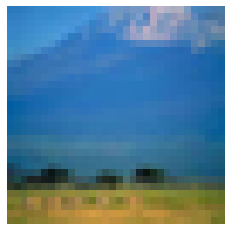
\includegraphics[width=.9\linewidth]{figs/fullimage.png}
        \subcaption{full image}
    \end{subfigure}
    \begin{subfigure}{.5\textwidth}
        \centering
        
\includegraphics[width=.9\linewidth]{figs/patchedimage.png}
        \subcaption{image divided in $12\times12=n$ patches}
    \end{subfigure}
    \caption{both figures are taken from the Keras vision transformer tutorial available at \url{https://keras.io/examples/vision/image_classification_with_vision_transformer/}}
    \label{img:patches}
\end{figure}



\section{ResNet}\label{sect:resnet}
As said before, we are going to combine both the architectures of ResNets and Transformers. While we have covered most of the concepts of the Transformers, we are still lacking the necessary concepts about ResNets. Let us start with the input of this architecture: an image $X\in\mathbb{R}^{C\times H \times W}$, where $C$ represents the number of channels, $H$ represents the image height and $W$ represents the image width.

The input image will go through a series of convolutional blocks. Each convolutional block is shown in Fig.~\ref{fig:convblock}. As you can see, the input (a tensor of dimension $C\times H \times W$) goes through convolutional layers an activation layer, and normalization layers. After this, the tensor is summed with the input and another activation is applied. One of the most important things to note is the skip connection named \texttt{id}. This type of connection, discovered to be effective by \cite{He16}, is responsible for improving performance, reduce the vanishing/exploding gradient problem, and smoothing the loss landscape \cite{Li17}. Following this simple structure, usually, a max-pooling layer is applied to reduce the number of features per channel. 

A full depiction of a resnet architecture is shown in Fig.~\ref{fig:resnet}. As you can see, many convolutional blocks are applied one after another increasing the number of channels from the original number (usually 3) to 512. The final depicted block is responsible for outputting the classification. 

\begin{figure}
    \begin{subfigure}{.61\textwidth}
        \centering
        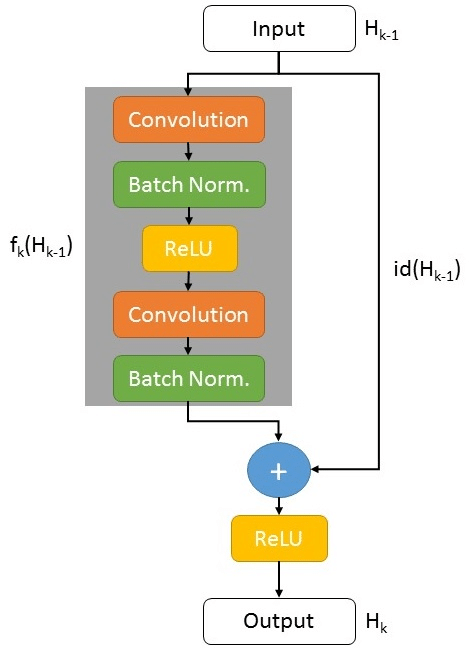
\includegraphics[width=.8\linewidth]{figs/convblock.png}
        \subcaption{Depiction of a convolutional block from \cite{Kumra17}}
        \label{fig:convblock}
    \end{subfigure}
    \begin{subfigure}{.5\textwidth}
        \centering
        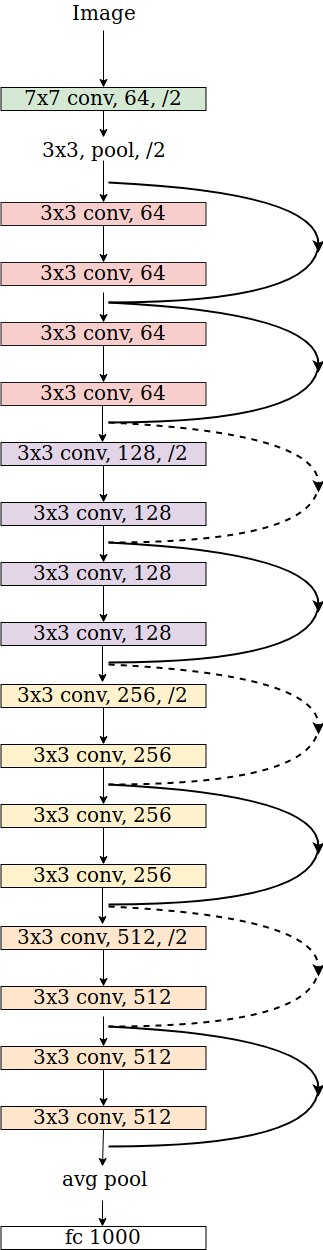
\includegraphics[width=.35\linewidth]{figs/resnet.png}
        \subcaption{Depiction of a ResNet from \cite{He16}}
        \label{fig:resnet}
    \end{subfigure}
\end{figure}


While the full intuition behind this architecture is extremely important it also out of the scope of this report. However, it is worth spending few more words about convolution. It is known that initial convolutional layers capture low-level features of the image e.g. lines, corners, and so on. Instead, higher convolutional layers use the low-level features to capture more and more abstract features like eyes, mouths, and so on.



\section{Dataset, Applications and Metrics}\label{sects:dataset}
\paragraph{Dataset}
In this section, we are going to discuss the dataset and the task that is proposed i.e. Facial Landmark Detection. Our dataset of choice is the 300W dataset \cite{Sagonas13a,Sagonas13b,Sagonas16}. Many other datasets are available, however, this one is one of the most popular. 300W comes already split into three parts: Test, Validation and Train each composed of $\sim 600,130,3700$ respectively. Each sample in the dataset is composed of an image and 68 landmark points on the image. The objective is to train a model to match the given points to the image. Fig.~\ref{img:sample} shows two examples.

\paragraph{Applications}
Facial landmark detection can be applied to a variety of important tasks. For example, \textit{face animation} and \textit{face reenactment} can both exploit the automatic generation of facial landmarks. Other important tasks are \textit{driver status tracking} and \textit{emotion classification} and \textit{face recognition} \cite{Khabarlak21}.

\begin{figure}
    \begin{subfigure}{.5\textwidth}
        \centering
        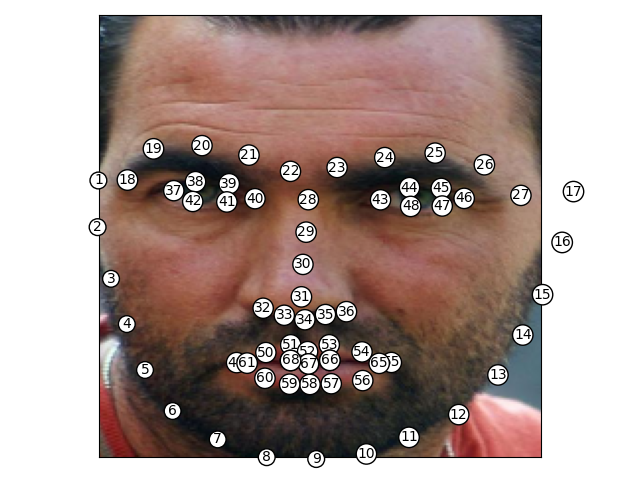
\includegraphics[width=.9\linewidth]{figs/sample1.png}
        \subcaption{Example 1}
    \end{subfigure}
    \begin{subfigure}{.5\textwidth}
        \centering
        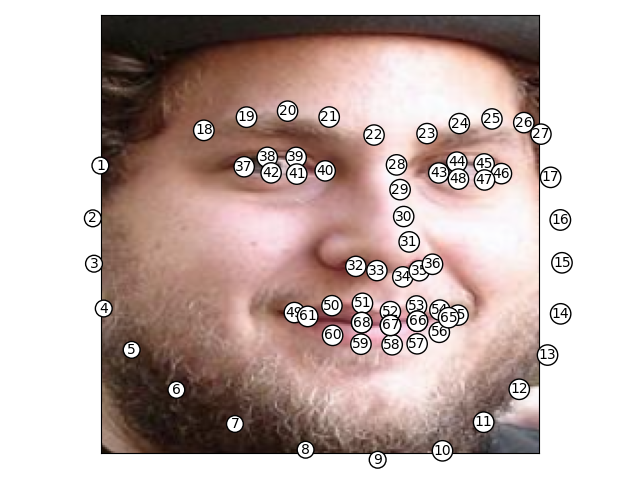
\includegraphics[width=.9\linewidth]{figs/sample2.png}
        \subcaption{Example 2}
    \end{subfigure}
    \caption{Two example with respective annotations from the 300W dataset}
    \label{img:sample}
\end{figure}


\paragraph{Metrics}
The goal of this task is to predict accurate landmarks on the human face. Therefore, a metric to measure the goodness of a model must take into account this fact. The most popular metric is the \textit{mean error}:
\[ME = \frac{1}{68}\sum_{i=1}^{68}||y_i-\hat{y_i}||\]
Where $y_i \in \mathbb{R}^2$ represents the prediction of i-th landmark and $\hat{y_i} \in \mathbb{R}^2$ represents the true i-th landmark position. Despite seeming perfectly reasonable as metric ME lacks an important normalization factor. In fact, An error of $10$ pixel in $4K$ images can be negligible while the same error on images of size $224\times 224$ can be considered a poor classification. To overcome this issue a normalization factor is introduced $d$. While the importance of $d$ is out of discussion there is not a true consensus among which normalization to adopt. In some cases, $d$ is the bounding box dimension, in other cases is the distance between the pupils but, most commonly, it is the distance between the 37-th landmark and 46-th landmark. In this report, we will consider only the latter.
\[NME = \frac{1}{68}\sum_{i=1}^{68}\frac{||y_i-\hat{y_i}||}{d}\]


\section{Combining ResNets with Transformers}\label{sect:architecture}

In this section we are going to discuss the chosen architecture. Firstly, we consider a pre-trained ResNet on ImageNet. In particular, ResNet101. We proceed by gaining access to different layers of the ResNet:

\begin{lstlisting}[language=Python]
self.resnet  = torchvision.models.resnet101(pretrained=True, progress=True)
self.resnet3 = torch.nn.Sequential(*list(self.resnet.children())[6:8])
self.resnet2 = torch.nn.Sequential(*list(self.resnet.children())[5:6])
self.resnet1 = torch.nn.Sequential(*list(self.resnet.children())[3:5])
self.resnet0 = torch.nn.Sequential(*list(self.resnet.children())[0:3])
...
res0 = self.resnet0(imgs)
res1 = self.resnet1(res0)
res2 = self.resnet2(res1)
res3 = self.resnet3(res2)
\end{lstlisting}

In the above listing, we split ResNet101 into four steps. These steps give us access to low-level and high-level features (\texttt{res0,res1,res2,res3}). These features will be fed to our Transformer Encoder. In particular, the sizes of these features are: $\text{imgs}\in\mathbb{R}^{b\times 3\times 224\times224}$, $\text{res}_0\in\mathbb{R}^{b\times64\times 112 \times 112}$, $\text{res}_1\in\mathbb{R}^{b\times256\times 56\times 56}$, $\text{res}_2\in\mathbb{R}^{b\times512\times 28\times 28}$, $\text{res}_3\in\mathbb{R}^{b\times2048 \times 7\times 7}$. Where $b$ represents the batch size. Next, we interpret these features as images. Thus, we can subdivide these images into patches.

\begin{lstlisting}[language=Python]
from einops import rearrange as r
res0 = r(res0,"b c (h1 h2) (w1 w2) -> b (c h1 w1) (h2 w2)",h1=2,w1=2)
res1 = r(res1,"b c (h1 h2) (w1 w2) -> b (c h1 w1) (h2 w2)",h1=2,w1=2)
res2 = r(res2,"b c (h1 h2) (w1 w2) -> b (c h1 w1) (h2 w2)",h1=2,w1=2)
res3 = r(res3,"b c h w -> b (h w) c")
\end{lstlisting}

Now, \texttt{res0,res1,res2} and \texttt{res3} contains more channels with linearized patches. Once again, it is worth looking at the shapes of these tensors. $\text{res}_0\in\mathbb{R}^{b\times1024\times784}$, $\text{res}_1\in\mathbb{R}^{b\times1024\times784}$, $\text{res}_2\in\mathbb{R}^{b\times2048\times196}$, $\text{res}_3\in\mathbb{R}^{b\times2048\times49}$. Now, it should not be too hard to interpret these linearized patches as tokens (much like in NLP) and feed them to a Transformer. However, there are two considerations to be made. Firstly, all patches sizes should be the same. To achieve this, we can employ a feed forward network. Secondly, we have $1024+1024+2048+2048=6144$ tokens which require too much memory. Thus, to reduce the memory footprint, we average several tokens togheter.

\begin{lstlisting}[language=Python]
from einops import reduce as rd
res0 = rd(ffB0(dropout(gelu(ffA0(res0)))),"b e (c1 c2)->b c1 e","max",c2=16)
res1 = rd(ffB1(dropout(gelu(ffA1(res1)))),"b e (c1 c2)->b c1 e","max",c2=8)
res2 = rd(ffB2(dropout(gelu(ffA2(res2)))),"b e (c1 c2)->b c1 e","max",c2=4)
res3 = rd(ffB3(dropout(gelu(ffA3(res2)))),"b e (c1 c2)->b c1 e","max",c2=1)
\end{lstlisting}

With the previous snippet, we solved the discussed issues. Now, we have a reasonable ammount of tokens (441) each one of them having the same size (512). We can concatenate these tokens togheter and proceed to add the positional embeddings.

\begin{lstlisting}[language=Python]
self.positions = torch.nn.Embedding(441,512).weight.unsqueeze(0)
...
srcs = torch.cat([res0,res1,res2,res3],1) 
srcs += self.positions.repeat(batch_size,1,1)
\end{lstlisting}

At this point, we have prepared the input for the transformer. We feed the prepared patches to the Transformer. Next, we can downscale the first $68$ tokens to only to $two$ features representing the landmark position on the face.

\begin{lstlisting}[language=Python]
from torch.nn import TransformerEncoder
from torch.nn import TransformerEncoderLayer
self.encoder = TransformerEncoder(
                    TransformerEncoderLayer(512,
                        nhead=8,
                        dim_feedforward=2048,
                        activation="gelu",
                        dropout=.1),
                    num_layers=4)
self.downscale = torch.nn.Linear(512,2)
...
mems = self.encoder(srcs.transpose(0,1)).transpose(0,1)
ldmk = self.downscale(mems[:,:68])
\end{lstlisting}

With this last piece, we have practically defined the entire architecture. The only thing remained to discuss is the training procedure. We used a \textit{l1 loss} with \textit{Adam} optimizer, \textit{learning rate} set to $1e^{-4}$ and \textit{batch size} of $32$.

Since the proposed dataset (300W) is quite small, we introduce three augmentation techniques. 
\begin{enumerate}
    \item random rotations.
    \item random crop.
    \item random jitter.
\end{enumerate}


\section{results}\label{sect:result}
In this section, we are going to show the results achieved by the proposed architecture in terms of normalized mean error (NME).
Table~\ref{table:results} shows the NME compared to other approaches. As you can see, our model is able to achieve results comparable with the state-of-the-art by achieving an NME of $4.26$. Compared to the best approach our architecture falls behind only of $1.13$. 

Next, we present two samples from the test set (see Fig.~\ref{fig:pred1} and ~\ref{fig:pred2}). As you can see, our model is capable of obtaining qualitative landmarks even with fairly complex expressions. 

\begin{table}\centering
    \begin{tabular}{lc}
        \toprule
        model & NME(\%) \\\midrule
        3DDE\cite{Valle19} & 3.13 \\
        CNNCRF\cite{Chen19} & 3.30 \\
        Adaloss\cite{Teixeira19} & 3.31 \\
        SAN-GT\cite{Dong18} & 3.98 \\
        ours & 4.26 \\
        CFSS\cite{Zhu16} & 5.76 \\
        \bottomrule
    \end{tabular}
    \caption{Results from various approaches for the same task \textit{facial landmarks detection}}
    \label{table:results}
\end{table}


\begin{figure}
    \begin{subfigure}{.61\textwidth}
        \centering
        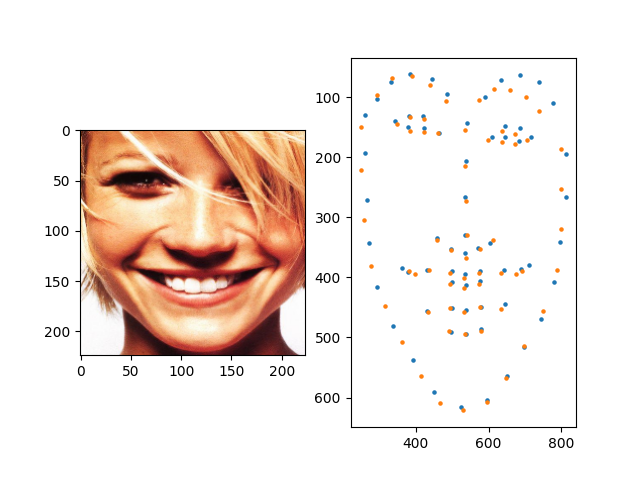
\includegraphics[width=.8\linewidth]{figs/prediction1.png}
        \subcaption{Example of prediction using our approach}
        \label{fig:pred1}
    \end{subfigure}
    \begin{subfigure}{.5\textwidth}
        \centering
        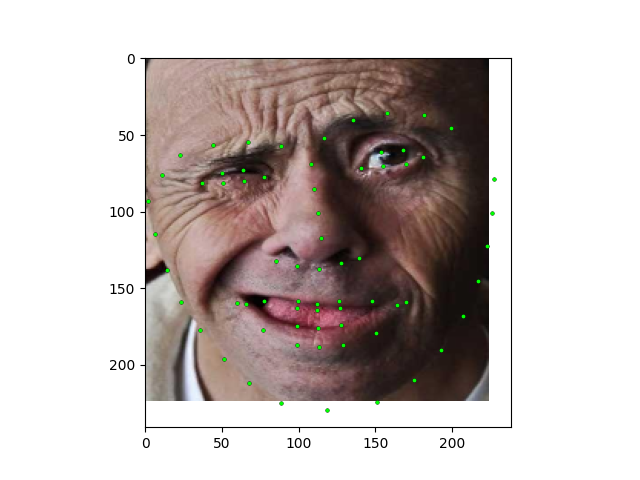
\includegraphics[width=.9\linewidth]{figs/prediction2.png}
        \subcaption{Second example of prediction using our approach}
        \label{fig:pred2}
    \end{subfigure}
    \caption{examples of predictions from the test set.}
    \label{figs:preds}
\end{figure}




\section{Conclusion \& Future Works}\label{sects:future}

In the last section, we have shown that a transformer can be used to achieve results close to the state-of-the-art for the task of Facial Landmark detection. Of course, many other things that could be done or improved to achieve better results. First of all, introducing more augmentation approaches could be beneficial. Secondly, deeper resnets and deeper transformer encoders could boost the performance. It could be worth trying other strategies to extract information from a resnet to be fed to a transformer.


\bibliographystyle{acm}
\bibliography{bibs/local.bib}
\end{document}
